
\section{Introduction} 
\label{sec:introduction}
	
	This machine learning master thesis is about neural networks (section \ref{sec:neural_networks}). 


	\subsection{Motivation}
		At the very beginning of this thesis, there is me, the writer. I wanted, from the very first day, to work on neural-networks and more specifically on deep-learning. I wanted so, because deep-learning has become in the last decade the most efficient algorithm at classifying images. 
		I was then searching for a topic. I discovered the work made by Ian J. Goodfellow, Jonathon Shlens and Christian Szegedy. In their publication named "Explaining and Harnessing Adversarial Examples"\cite{goodfellow2014explaining} they motivate that adversarial learning could improve the accuracy of some given neural-networks. After contacting one of the authors of this publication, it appeared that it would be a good contribution to validate their observations on other datasets, since most of their test are based on the MNIST dataset\cite{lecun-mnist}. Therefore, the following thesis is about further validating the proposed adversarial-learning method described in \cite{goodfellow2014explaining} with different datasets.

	\subsection{Methodology}
		We are therefore going to investigate on how is adversarial-learning performing with shallow-neural-networks on different datasets. On the same time, we are going to investigate on the reasons underlining this performances. To do so, we will first re-implement the proposed solution of \cite{goodfellow2014explaining} in such a way that we isolate adversarial-learning from other techniques used in the paper. At this point we will emphasize the benefits of adversarial-learning. 

		We will then move to another dataset similar to the first one, there will also be 10 different classes of images to classify. That dataset will be the CIFAR10\cite{CIFAR10_BITCHES}. Again, some knowledge will be acquired from this experience. Finally, we will test the adversarial-learning on a dataset of other nature. The one we would try is a phoneme dataset: the TIMIT dataset\cite{maybe...}. The results obtained from this dataset will further validate the technique as useful for classification in the context of shallow-neural-network.

	\subsection{Expected outcome}
		In their paper, Ian J. Goodfellow, Jonathon Shlens and Christian Szegedy, described their technique to able to ??? 
		=> How adversarial learning best separate the classes.
		With this adversarial-learning technique we expect to have a network able to emphasize the differences the classes. We expect the network to learn the differences between classes more than just the pattern of a class.


	\subsection{Adversarial-learning}
		Until now, we've been teasing adversarial-learning without explaining what it is about. Lets start off with mentioning what an adversarial sample to a classifier would be. Imagine you have full knowledge of a given classifier. Starting from there, you can create samples to this classifier that are going to give some predictions. Knowing how does the classifier behaves, you can creates samples leading your classifier to some mistakes. This are adversarial samples. In machine learning, adversarial-learning is about creating a classifier resisting to adversarial samples.

		In the publication that interest us\cite{goodfellow2014explaining}, the authors noticed that twisting each pixels of the input images by some very specific values (the adversarial values), an accurate classifier could be easily fooled. Lets detail : Consider you have a classifier able to recognize the MNIST dataset and this classifier makes 10 errors when guessing the classes of 200 samples. Now, if you modify each pixels of these 200 samples by a little value, the classifier makes 180 errors. You've fooled your classifier. 

		The adversarial-learning algorithm we use, is going to embed some properties letting the classifier resist to some adversarial samples. More specifically, we are going to train our classifier on adversarial samples that could have been used to fool our classifier.



	\subsection{Setting-up an example}
		To understand our adversarial training we will use a simple neural network composed by two sigmoid neurons (see section \ref{sec:Artificial_neurons}). The network aims a recognizing a columns and a dot in a three by one pixels image. This network is sketched on \fref{fig:2N_NN}. Considering a white pixel has value $1$ and a dark pixel has value $0$, a column could be represented by a vector $x^1 = [1,0,1]$ and a dot could be by $x^2 = [0,0,1]$. We consider the column to be the output $y^i = 0$ and the dot to be the output $y^i = 1$
		To predict a sensible value, a two-sigmoid network could use the weights and biases :
		$$ W = \left( \begin{matrix} 1 & -1 \\ -1 & -1 \\ 1 & 1 \end{matrix} \right) ; b = \left( \begin{matrix} -1.5 & 0.5 \end{matrix} \right)$$
		
		\vskip 1em
		\textbf{signal propagation: } The input signal $x^i$ propagates through the network resulting in a prediction vector $p^i = \sigma(W^Tx + b)$. To know how right or wrong is this prediction vector, we would use a cost function like the negative log-likelihood:
		$$ C^i = y^i \ln(p^i) + (1-y^i)\ln(1-p^i) $$
		Propagating $x^1$ and $x^2$, we get that $p^1 = [\sigma(.5), \sigma(-.5)]$ and $p^2 = [\sigma(-.5), \sigma(.5)]$

		\begin{figure}
			\centering
			\def\layersep{1.5cm}	
			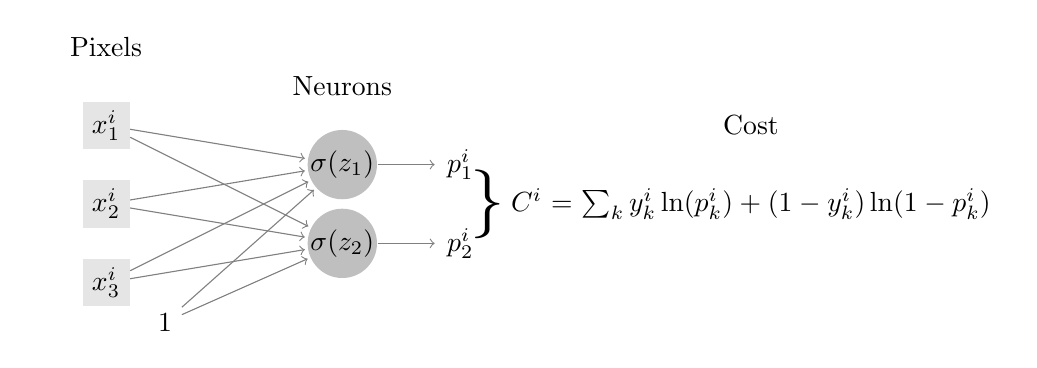
\begin{tikzpicture}[shorten >=1pt,->,draw=black!50, node distance=\layersep]
			    \tikzstyle{every pin edge}=[<-,shorten <=1pt]
			    \tikzstyle{pixel} = [rectangle, fill=black!10,minimum size=17pt,inner sep=0pt]
			    \tikzstyle{neuron}=[circle,fill=black!25,minimum size=17pt,inner sep=0pt]
			    \tikzstyle{annot} = [text width=5em, text centered]
			    \tikzstyle{annot2} = [text width=18em, text centered]
				\tikzstyle{accolade} = [rectangle, text centered, minimum size=17pt]
			    
			    %%% DRAW THE NODES
			    \foreach \name / \y in {1,2,3}
			        \node[pixel] (I-\name) at (0,-\y) {$x^i_\y$};
			    \node[] (I-4) at (\layersep/2,-3.5) {$1$};
			    \foreach \name / \y in {1,2}
					\node[neuron] (O-\y) at (\layersep*2,-\y-0.5) {$\sigma(z_\y)$};
				\foreach \name / \y in {1,2}	
					\node[] (C-\y) at (\layersep*3,-\y-0.5) {$p^i_\y$};

			    %%% DRAW THE PATHS
			    \foreach \source in {1,...,4}
			        \foreach \dest in {1,2}
			            \path (I-\source) edge (O-\dest);
			    \foreach \y in {1,2}
			        \path (O-\y) edge (C-\y);

			    %%% ANOTATE
			    \node[accolade] at (\layersep*3+1em,-2) { \Huge\} };
			    \node[annot2] at (\layersep*3+10.5em,-2) (cost) {$C^i = \sum_k y^i_k \ln(p^i_k) + (1-y^i_k)\ln(1-p^i_k) $};

			    \node[annot,above of=I-1, node distance=1cm] (iv) {Pixels};
			    \node[annot,above of=O-1, node distance=1cm] (iv) {Neurons};
			    \node[annot,above of=cost, node distance=1cm] (iv) {Cost};

			\end{tikzpicture}
			\label{fig:2N_NN}
			\caption{Two neurons neural network}
		\end{figure}


	\subsection{Adversarial learning}
		Imagine you are allowed to modify each pixels of our image by a value $\epsilon$. Intuitively, if you want to improve the recognition, you would increase the contrast in the picture and insist on the dots where the aught to be. On the other hand, if you want to confuse the recognition, you would lower the contrast and add color where there shouldn't be.

		These properties are the ones we aught to enforce with our adversarial learning. For an epsilon small enough, we subtract to $x^i$ $\epsilon$ times the sign of the derivative with respect to $x^i$ of the Cost $C^i$.
		$$ x^{i_{\text{adv}}} \leftarrow x^i - \epsilon \text{ sign}(\nabla_{x^i} C^i) $$
		Therefore the input $x^i$ is modified such that ?? TODO: HERE IS THE THING ??

		\vskip 1em
		\textbf{In our example. } We apply the adversarial learning to our example. First we compute the derivative of the Cost with respect to $x^i$. (The mathematics behind this derivative is detailed on the appendix \ref{sec:2N_NN_cost})
		$$	\frac{\delta C^i}{\delta x^i} = W \cdot \left( y^i -p^i \right) $$
		Then we subtract the sign of this derivative to the actual input $x^i$
		\begin{equation}
			\begin{split}
				x^{1_{\text{adv}}} &\leftarrow x^1 - \epsilon \text{ sign}(\nabla_{x^1} C(W,b,x^1)) \\
				x^{1_{\text{adv}}} &\leftarrow x^1 - \epsilon \text{ sign}( W \cdot ( y^i -p^i) )
			\end{split}
		\end{equation}
		\begin{equation}
			x^1 = \left( \begin{matrix} 1 \\ 0 \\ 1 \end{matrix} \right) ;
			x^{1_{\text{adv}}} = \left( \begin{matrix} .7 \\ 0 \\ 1 \end{matrix} \right) ;
			x^2 = \left( \begin{matrix} 0 \\ 0 \\ 1 \end{matrix} \right) ;
			x^{2_{\text{adv}}} = \left( \begin{matrix} .3 \\ 0 \\ 1 \end{matrix} \right) ;
		\end{equation}
		


		Once we have these derivatives, the worst modification we can make to sample $x^i$ is by following this derivative. 
		

	\subsection{Dataset}
		The first dataset we will be using is the MNIST\ref{??} dataset. This dataset is composed by 60k gray scale images. Each of them represent a hand written digit (6k of each). 







		